\chapter{Arhitektura i dizajn sustava}
		
		Arhitektura ovog sustava je bazirana na arhitekturi klijent-poslužitelj. Sustav se sastoji od 3 sloja: sloj korisničkog sučelja, sloj aplikacijske logike, sloj podataka.
		
		\textbf{Web preglednik} je program preko kojeg korisnik koristi aplikaciju. Preglednik omogućuje klijentu komunikaciju s web poslužiteljem aplikacije. Preglednik nam omogućava prikaz sloja korisničkog sučelja sustava. Korisnik preko web preglednika komunicira s web poslužiteljem slanjem i primanjem HTTP zahtjeva. Primljene podatke i datoteke web preglednik zna interpretirati i prikazati korisniku tako da sama interakcija s aplikacijom bude jednostavna. Neki od popularnih web preglednika su Crome, Safari i Edge.
		
		\textbf{Web poslužitelj} je računalo na kojem se aplikacija pokreće. Na njemu se dakle nalazi sloj aplikacijske logike. Web poslužitelj aplikaciji prosljeđuje zahtjeve na obradu i njezine odgovore prosljeđuje natrag klijentima. Web aplikacija na poslužitelju obrađuje zaprimljene zahtjeve. Ako obrada zahtjeva to zahtjeva, web aplikacija dodatno komunicira sa slojem podataka.
		
		\textbf{Baza Podataka} predstavlja sloj podataka. U bazi podataka se na siguran način spremaju svi podaci koje je potrebno trajno čuvati. To podrazumijeva podatke o prijavama, korisničkim računima i slično. Takvi podaci moraju ostati očuvani i ako je rad aplikacije prekinut iz bilo kojeg razloga. Baza podataka je detaljnije opisana u poglavlju  \ref{sec:bazaPodataka}.
		
		\textbf{Web aplikacija} je podijeljena na frontend i backend.
		
		\textbf{Frontend} je zapravo prezentacijski dio aplikacije i zadužen je za interakciju s korisnikom. On oblikuje korisničko sučelje i samim time definira što će korisnik vidjeti na web pregledniku kada koristi aplikaciju.
		
		\textbf{Backend} je dio aplikacije koji obrađuje zahtjeve i kontrolira rad ostalih dijelova sustava. Baceknd je usko povezan sa web poslužiteljem.
		
		Za izradu backend dijela aplikacije odabrali smo programski jezik Java s radnim okvirom Spring Boot. Spring Boot radni okvir koristi višeslojnu arhitekturu u kojoj svaki sloj komunicira sa slojem koji se u hijerarhiji nalazi iznad ili ispod njega. Arhitektura Spring Boota se sastoji od četiri sloja:
		\begin{packed_item}
			\item \textbf{Prezentacijski sloj} (\textit{Presentation layer}) - Ovo je najviši sloj arhitekture i predstavlja frontend dio aplikacije. Ovaj sloj prima HTTP zahtjeve i vrši autentifikaciju. Također vrši pretvorbu JSON objekata u objekte u Javi i obrnuto. Na kraju svoje obrade Prezentacijski sloj prosljeđuje HTTP zahtjev sljedećem sloju.
			
			\item \textbf{Poslovni sloj} (\textit{Business layer}) - Ovaj sloj sadrži svu poslovnu logiku te je zadužen za validaciju i autorizaciju.
			
			\item \textbf{Sloj postojanosti} (\textit{Persistence layer}) - Ovaj sloj sadrži logiku vezanu uz pohranu u bazu podataka. Sloj pretvara zapise iz baze podataka u objekte iz poslovnog sloja i obrnuto.
			
			\item \textbf{Sloj baze podataka} (\textit{Database layer}) - Ovaj sloj sadrži 	bazu podataka ili više njih. Sloj je zadužen za obavljanje CRUD (copy, read, update, delete) operacija.
		\end{packed_item}
		
		\begin{figure}[H]
			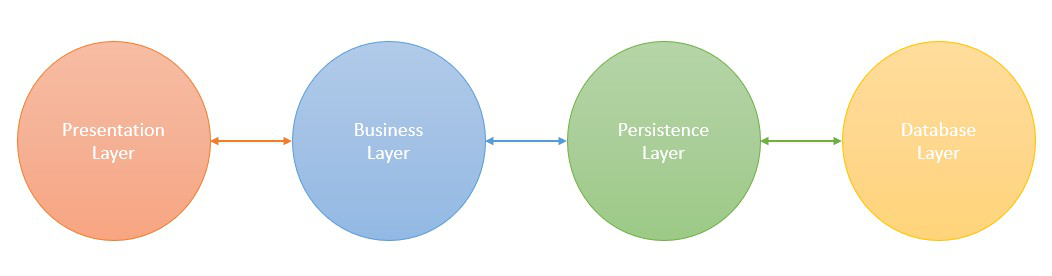
\includegraphics[width=\textwidth]{slike/slojeviArhitekture.jpg} %veličina u odnosu na širinu linije
			\caption{Prikaz Spring Boot arhitekture}
			\label{fig:MVC1} %label mora biti drugaciji za svaku sliku
		\end{figure}
		
		Za razvoj frontend dijela aplikacije odlučili smo koristiti programski jezik JavaScript uz radni okvir React. React omogućuje jednostavanu izradu korisničkog sučelja preko JavaScripta, bez direktnog korištenja HTML-a.
		
	\eject
	
		\section{Baza podataka}
		\label{sec:bazaPodataka}
		
		Ovaj sustav će za svoje potrebe koristiti relacijsku bazu podataka implementirana u PostgreSQL-u. Ovakav tip baze podataka svojom strukturom omogućuje jednostavno modeliranje elemenata iz stvarnog svijeta i zbog toga je široko primjenjiv. Odabrali smo implementaciju u PostgreSQL-u jer smo s ovom implementacijom već dobro upoznati. Relacijske baze podataka se sastoje od relacija. Relacije su predstavljene tablicama koje su definirane svojim nazivom i skupom atributima. Bazu podataka koristimo za jednostavnu i sigurnu pohranu, izmjenu, umetanje i dohvat podataka potrebnih za rad sustava. Naša baza podataka se sastoji od sljedećih relacija, odnosno tablica:
		
		\begin{packed_item}
			\item Users
			\item Report
			\item Image
			\item Category
			\item CategoryKeywords
			\item ReportGroup 
			\item Feedback
			\item CityOffice
		\end{packed_item}
		
			\subsection{Opis tablica}
			
			\textbf{Users} tablica čuva podatke o korisničkim računima koje korisnici izrađuju tijekom registracije. Tablica je povezana vezom \textit{One-to-Many} s tablicom \textit{Report} preko atributa \textit{userID}.
			
			\begin{longtblr}[
					label=Users,
					entry=none
				]{
					width = \textwidth,
					colspec={|X[6,l]|X[6, l]|X[20, l]|}, 
					rowhead = 1,
				} %definicija širine tablice, širine stupaca, poravnanje i broja redaka naslova tablice
				\hline \SetCell[c=3]{c}{\textbf{Users}}	 \\ \hline[3pt]
				\SetCell{LightGreen} userID & INT & jedinstveni identifikator korisnika \\ \hline
				email & VARCHAR & email adresa korisnika \\ \hline 
				firstName & VARCHAR & ime korisnika \\ \hline
				lastName & VARCHAR & prezime korisnika \\ \hline 
				password & VARCHAR & kriptirana lozinka za korisnički račun \\ \hline 
			\end{longtblr}
			
			\textbf{Report} tablica čuva podatke o pojedinim prijavama oštećenja koje korisnici podnose. Tablica je povezana vezom \textit{Many-to-One} s tablicom \textit{Users} preko atributa \textit{userID}, \textit{Many-to-One} vezom s tablicom \textit{Category} preko atributa \textit{categoryID} i \textit{Many-to-One} vezom s tablicom ReportGroup preko atributa groupID.
			
			\begin{longtblr}[
				label=Report,
				entry=none
				]{
					width = \textwidth,
					colspec={|X[8,l]|X[6, l]|X[20, l]|}, 
					rowhead = 1,
				} %definicija širine tablice, širine stupaca, poravnanje i broja redaka naslova tablice
				\hline \SetCell[c=3]{c}{\textbf{Report}}	 \\ \hline[3pt]
				\SetCell{LightGreen} reportID & INT & jedinstveni identifikator prijave \\ \hline
				location & VARCHAR & lokacija oštećenja \\ \hline
				description & VARCHAR & opis oštećenja \\ \hline 
				reportTS & TIMESTAMP & vrijeme prijave \\ \hline 
				reportHeadline & VARCHAR & naslov prijave \\ \hline 
				\SetCell{LightBlue} userID & INT & jedinstveni identifikator korisnika koji je podnio prijavu \\ \hline 
				\SetCell{LightBlue} categoryID & INT & jedinstveni identifikator kategorije oštećenja \\ \hline
				\SetCell{LightBlue} groupID & INT & jedinstveni identifikator grupe prijave \\ \hline
			\end{longtblr}
			
			\textbf{Image} tablica čuva podatke o slikama koje se prilažu u prijavama oštećenja. Tablica je povezana \textit{Many-to-One} vezom s tablicom \textit{Report} preko atributa \textit{reportID}.
			
			\begin{longtblr}[
				label=Image,
				entry=none
				]{
					width = \textwidth,
					colspec={|X[6,l]|X[6, l]|X[20, l]|}, 
					rowhead = 1,
				} %definicija širine tablice, širine stupaca, poravnanje i broja redaka naslova tablice
				\hline \SetCell[c=3]{c}{\textbf{Image}}	 \\ \hline[3pt]
				\SetCell{LightGreen} imageID & INT & jedinstveni identifikator slike \\ \hline
				\SetCell{LightBlue} reportID & INT & jedinstveni identifikator prijave kojoj slika pripada \\ \hline
				URL & VARCHAR & URL slike \\ \hline 
			\end{longtblr}
			
			\textbf{Category} tablica čuva podatke o kategorijama kojima oštećenje može pripadati. Tablica je povezana \textit{One-to-Many} vezom s tablicom \textit{Report} preko atributa \textit{categoryID}, \textit{Many-to-One} vezom s tablicom \textit{CityOffice} preko atributa \textit{cityOfficeID} i \textit{One-to-Many} vezom s tablicom \textit{CategoryKeywords} preko atributa \textit{categoryID}.
			
			\begin{longtblr}[
				label=Category,
				entry=none
				]{
					width = \textwidth,
					colspec={|X[6,l]|X[6, l]|X[20, l]|}, 
					rowhead = 1,
				} %definicija širine tablice, širine stupaca, poravnanje i broja redaka naslova tablice
				\hline \SetCell[c=3]{c}{\textbf{Category}}	 \\ \hline[3pt]
				\SetCell{LightGreen} categoryID & INT & jedinstveni identifikator kategorije \\ \hline
				categoryName & VARCHAR & naziv kategorije \\ \hline 
				\SetCell{LightBlue} cityOfficeID & INT & jedinstveni identifikator gradskog ureda koji obrađuje prijave oštećenja iz ove kategorije \\ \hline
			\end{longtblr}

			\textbf{CategoryKeywords} tablica čuva podatke o ključnim riječima po kojima se može identificirati kategorija oštećenja. Tablica je povezana \textit{Many-to-One} vezom s tablicom \textit{Category} preko atributa \textit{categoryID}.

			\begin{longtblr}[
				label=CategoryKeywords,
				entry=none
				]{
					width = \textwidth,
					colspec={|X[6,l]|X[6, l]|X[20, l]|}, 
					rowhead = 1,
				} %definicija širine tablice, širine stupaca, poravnanje i broja redaka naslova tablice
				\hline \SetCell[c=3]{c}{\textbf{CategoryKeywords}}	 \\ \hline[3pt]
				\SetCell{LightGreen} keywordID & INT & jedinstveni identifikator ključne riječi \\ \hline
				keyword & VARCHAR & ključna riječ \\ \hline 
				\SetCell{LightBlue} categoryID & INT & jedinstveni identifikator kategorije kojoj ključna riječ pripada. \\ \hline
			\end{longtblr}
			
			\textbf{ReportGroup} tablica predstavlja grupu prijava koje su objedinjene. Tablica je povezana \textit{One-to-Many} vezom s tablicom \textit{Report} preko atributa \textit{groupID} i \textit{One-to-Many} vezom s tablicom \textit{Feedback} preko atributa \textit{groupID}.
			
			\begin{longtblr}[
				label=ReportGroup,
				entry=none
				]{
					width = \textwidth,
					colspec={|X[6,l]|X[6, l]|X[20, l]|}, 
					rowhead = 1,
				} %definicija širine tablice, širine stupaca, poravnanje i broja redaka naslova tablice
				\hline \SetCell[c=3]{c}{\textbf{ReportGroup}}	 \\ \hline[3pt]
				\SetCell{LightGreen} groupID & INT & jedinstveni identifikator grupe prijava \\ \hline
			\end{longtblr}
			
			\textbf{Feedback} tablica čuva podatke o statusu pojedine grupe prijava. Također čuva podatke potrebne za slanje povratnih informacija korisnicima i računanje nekih statistika. Tablica je povezana \textit{Many-to-One} vezom s tablicom \textit{ReportGroup} preko atributa \textit{groupID} i \textit{Many-to-One} vezom s tablicom \textit{CityOffice} preko atributa \textit{cityOfficeID}.
			
			\begin{longtblr}[
				label=Feedback,
				entry=none
				]{
					width = \textwidth,
					colspec={|X[6,l]|X[6, l]|X[20, l]|}, 
					rowhead = 1,
				} %definicija širine tablice, širine stupaca, poravnanje i broja redaka naslova tablice
				\hline \SetCell[c=3]{c}{\textbf{Feedback}}	 \\ \hline[3pt]
				\SetCell{LightGreen} cityOfficeID & INT & jedinstveni identifikator gradskog ureda \\ \hline
				\SetCell{LightGreen} groupID & INT & jedinstveni identifikator grupe prijava na koju se podaci referiraju \\ \hline
				status & VARCHAR & status prijava u referiranoj grupi \\ \hline 
				changeTS & TIMESTAMP & vrijeme kada se postavio status prijava iz referirane grupe \\ \hline
			\end{longtblr}
			
			\textbf{CityOffice} tablica čuva podatke o računima gradskih ureda. Tablica je povezana \textit{One-to-Many} vezom s tablicom \textit{Feedback} preko atributa \textit{cityOfficeID} i \textit{One-to Many} vezom s tablicom \textit{Category} preko atributa \textit{cityOfficeID}.
			
			\begin{longtblr}[
				label=CityOffice,
				entry=none
				]{
					width = \textwidth,
					colspec={|X[10,l]|X[6, l]|X[20, l]|}, 
					rowhead = 1,
				} %definicija širine tablice, širine stupaca, poravnanje i broja redaka naslova tablice
				\hline \SetCell[c=3]{c}{\textbf{CityOffice}}	 \\ \hline[3pt]
				\SetCell{LightGreen} cityOfficeID & INT & jedinstveni identifikator gradskog ureda \\ \hline
				cityOfficeName & VARCHAR & naziv gradskog ureda \\ \hline
				cityOfficeEmail & VARCHAR & email adresa gradskog ureda \\ \hline 
				cityOfficePassword & VARCHAR & kriptirana lozinka za račun gradskog ureda \\ \hline
			\end{longtblr}
			
			\subsection{Dijagram baze podataka}
			
			\begin{figure}[H]
				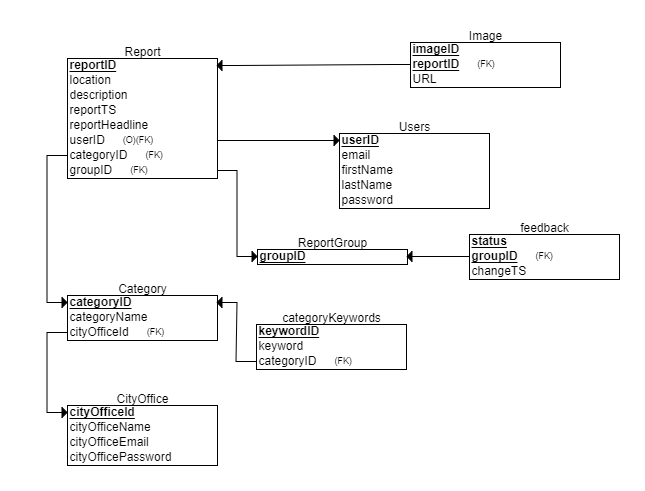
\includegraphics[width=\textwidth]{slike/relacijski.png} %veličina u odnosu na širinu linije
				\caption{Relacijski dijagram baze podataka}
				\label{fig:DijagramBazePodataka} %label mora biti drugaciji za svaku sliku
			\end{figure}
			
			\eject
			
			
		\section{Dijagram razreda}
		
			Na slikama \ref{fig:kontroler}, \ref{fig:dao}, \ref{fig:repo}, \ref{fig:service} su prikazani razredi koji pripadaju backend dijelu aplikacije. Razredi su arhitekturom podijeljeni na kontrolere, repozitorije i servise. Također postoje Domain i DTO (Data Transfer Object) modeli.
		
			Slika \ref{fig:kontroler} prikazuje klase koje imaju ulogu kontrolera, tj. u kodu imaju anotaciju @RestController. Te klase definiraju endpointove i koriste se za dohvat i manipuliranje podacima iz baze podataka. Klase sa @RestController anotacijom koriste instance servisa. Servisi su klase koje imaju @Service anotaciju. Servisi implementiraju metode za upis (npr. createUser(Users);, createCitiyOffice(cityOffice), itd.), brisanje, dohvat i izmjenu podataka u bazi. Klasa ServerApplication je glavna klasa koja pokreće aplikaciju, a ServerApplicationTest služi za testiranje funkcionalosti aplikacije.
		
			\begin{figure}[H]
				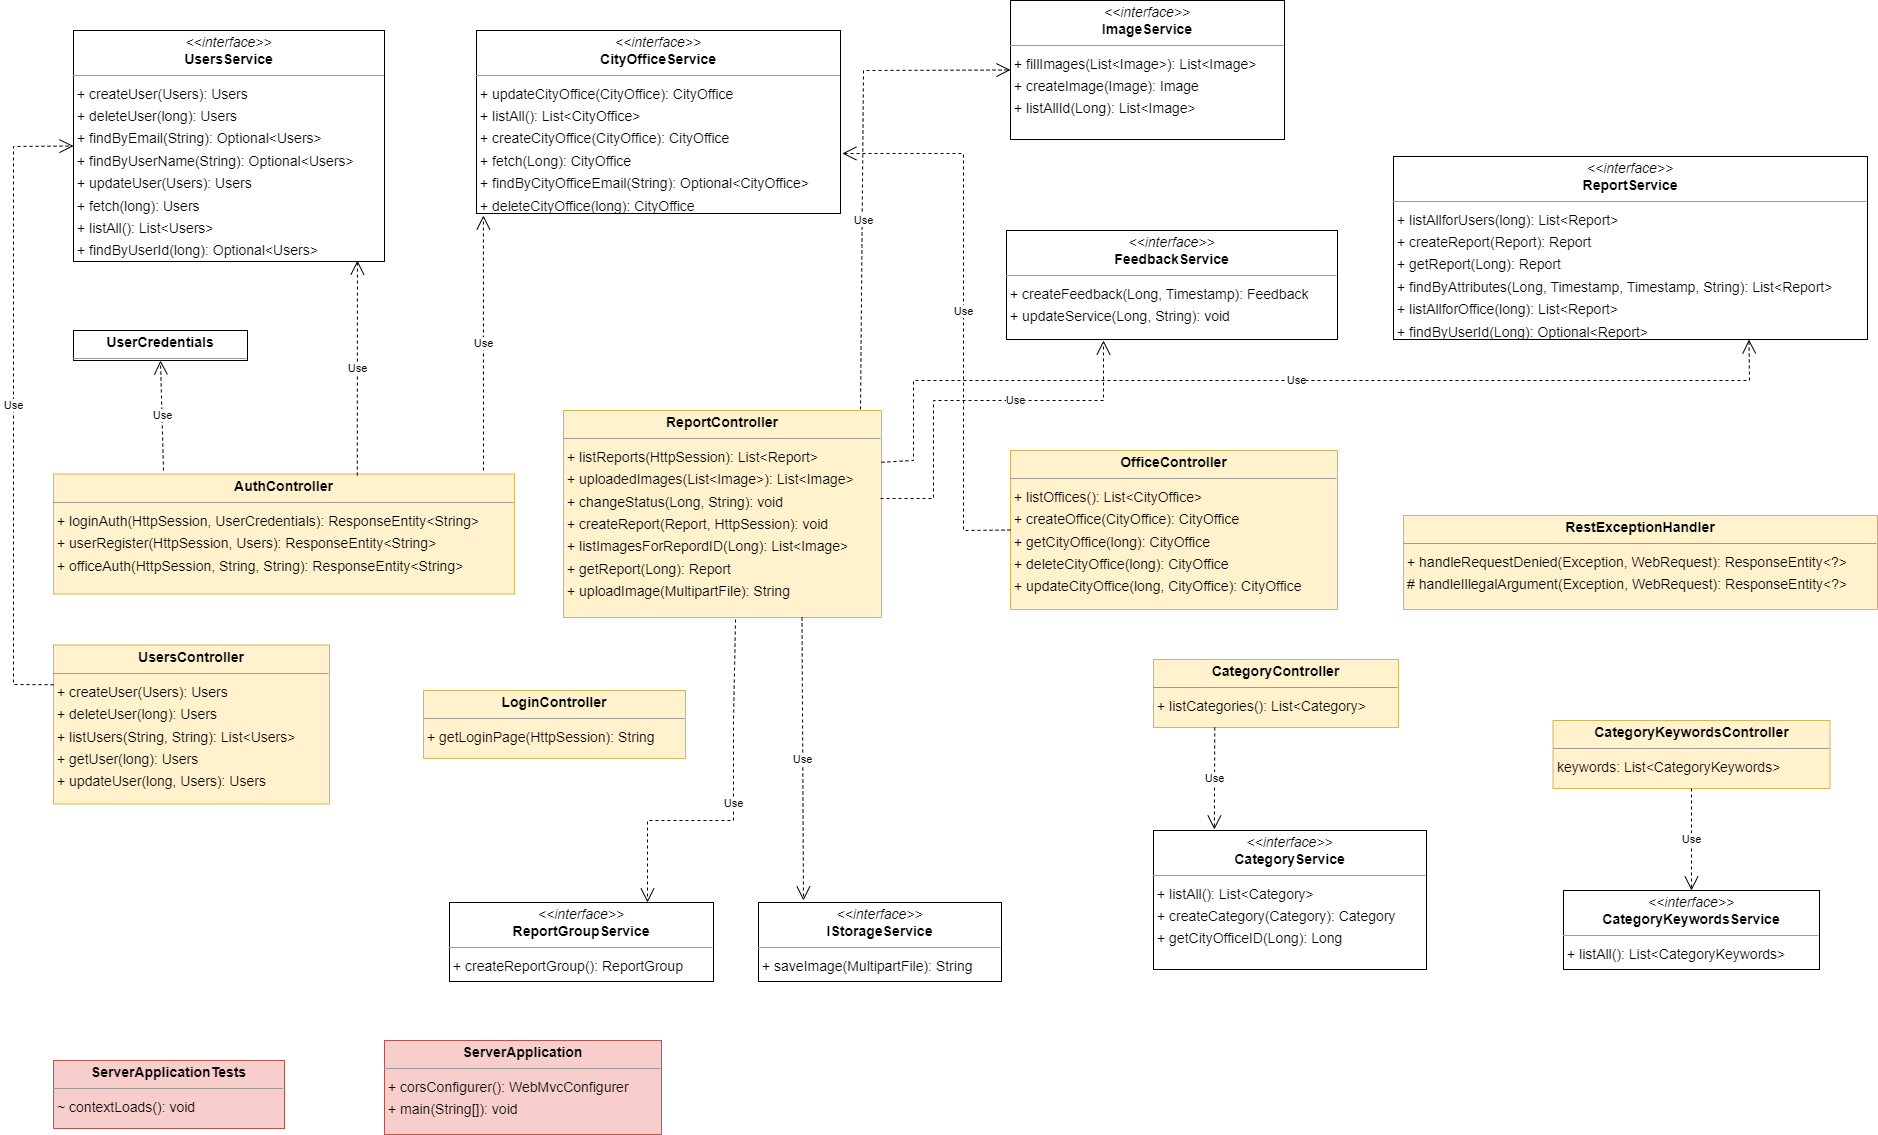
\includegraphics[width=\textwidth]{slike/controller.png} %veličina u odnosu na širinu linije
				\caption{Kontroleri na backendu}
				\label{fig:kontroler} %label mora biti drugaciji za svaku sliku
			\end{figure}
			
			\eject
			
			Slika \ref{fig:dao} prikazuje sučelja koja nasljeđuju sučelje JpaRepository. Sučelje JpaRepository definira razne CRUD (create, read, update, delete) metode za rad nad entitetima u bazi. Definirane metode izvršavaju razne vrste upite nad bazom podataka.
			
			\begin{figure}[H]
				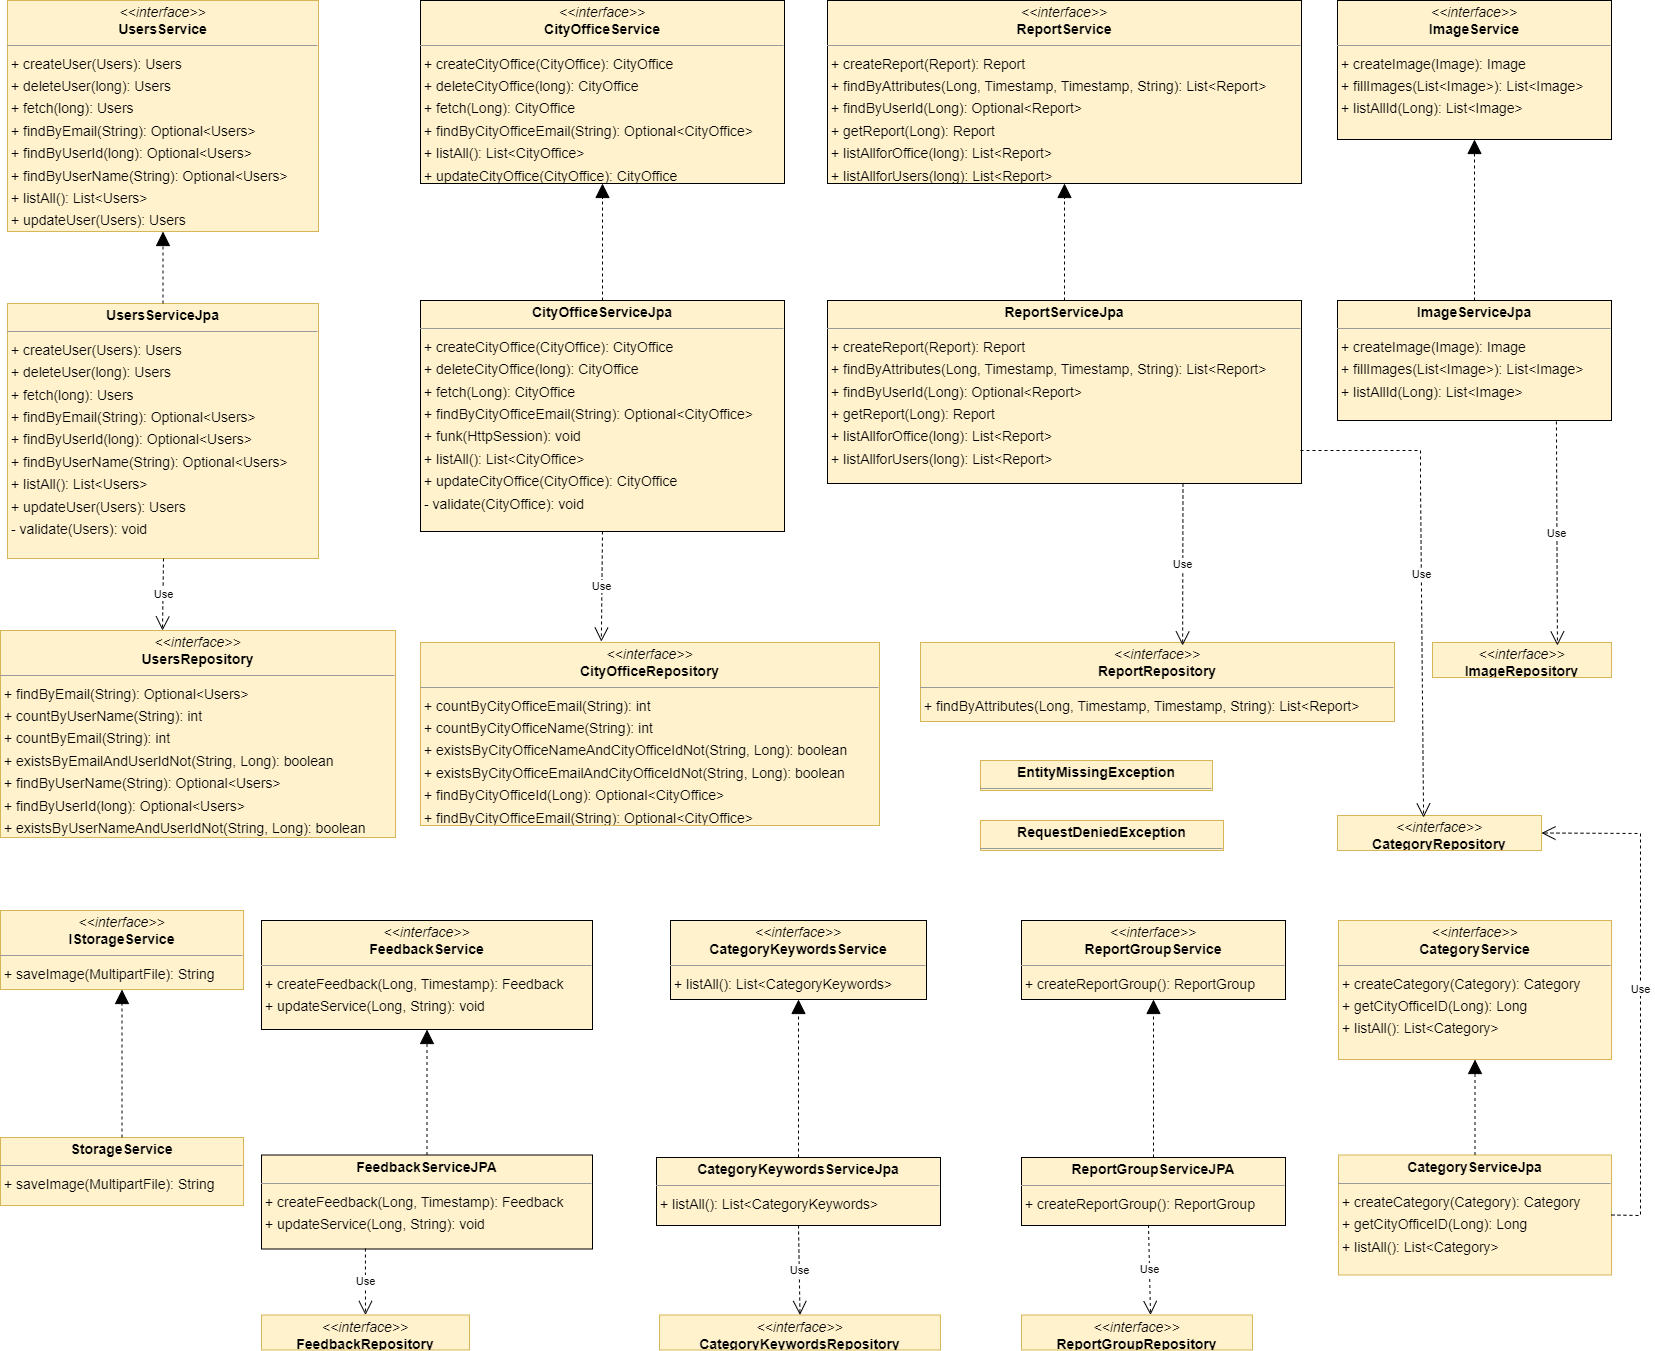
\includegraphics[width=\textwidth]{slike/dao.png} %veličina u odnosu na širinu linije
				\caption{Data Access Objects}
				\label{fig:dao} %label mora biti drugaciji za svaku sliku
			\end{figure}
			
			\eject
			
			Slika \ref{fig:repo} prikazuje klase u paketu repo koje reprezentiraju entitete u bazi podataka te njihove međusobne veze. Ove klase definiraju tipove atributa pojedinih entiteta, ograničenja nad atributima i primarne i strane ključeve. Svaka klasa ima implementirane metode get() i set() za svaki od atributa, kao i odgovarajuće konstruktore. Klasa FeedbackID služi kao pomoćna klasa za definiranje primarnog ključa feedback. Korisnici (Users) stvaraju prijave (Report), a gradski uredi (CityOffice) upravljaju prijavama i prilikom promjena automatski zapisuje nove povratne informacije (Feedback) u bazu podataka za tu grupu prijava.
			
			\begin{figure}[H]
				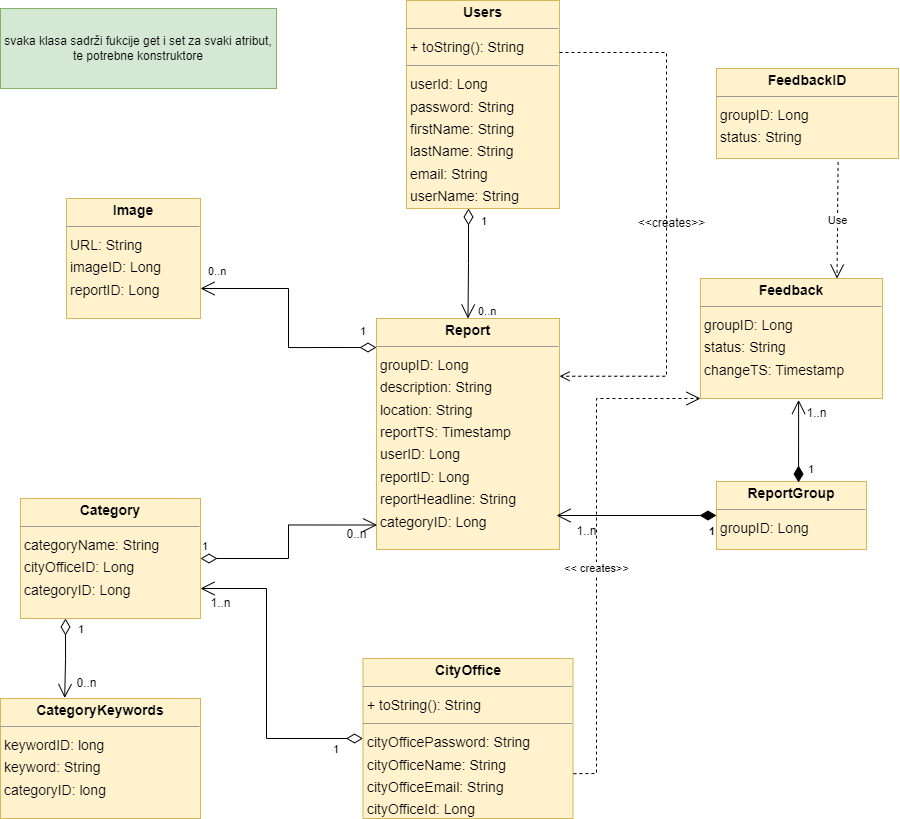
\includegraphics[width=\textwidth]{slike/repo.png} %veličina u odnosu na širinu linije
				\caption{Modeli}
				\label{fig:repo} %label mora biti drugaciji za svaku sliku
			\end{figure}
			
			\eject
			
			Slika \ref{fig:service} prikazuje klase servisa koje definiraju metode za CRUD operacije nad bazom podataka. EntityMissingException i RequestDeniedException su pomoćne klase za baratanje pogreškama. Klase servisa koriste instance Repository klasa iz slike 2. za poziv metoda definiranih u sklopu sučelja Repository odnosno JpaRepository.
			
			\begin{figure}[H]
				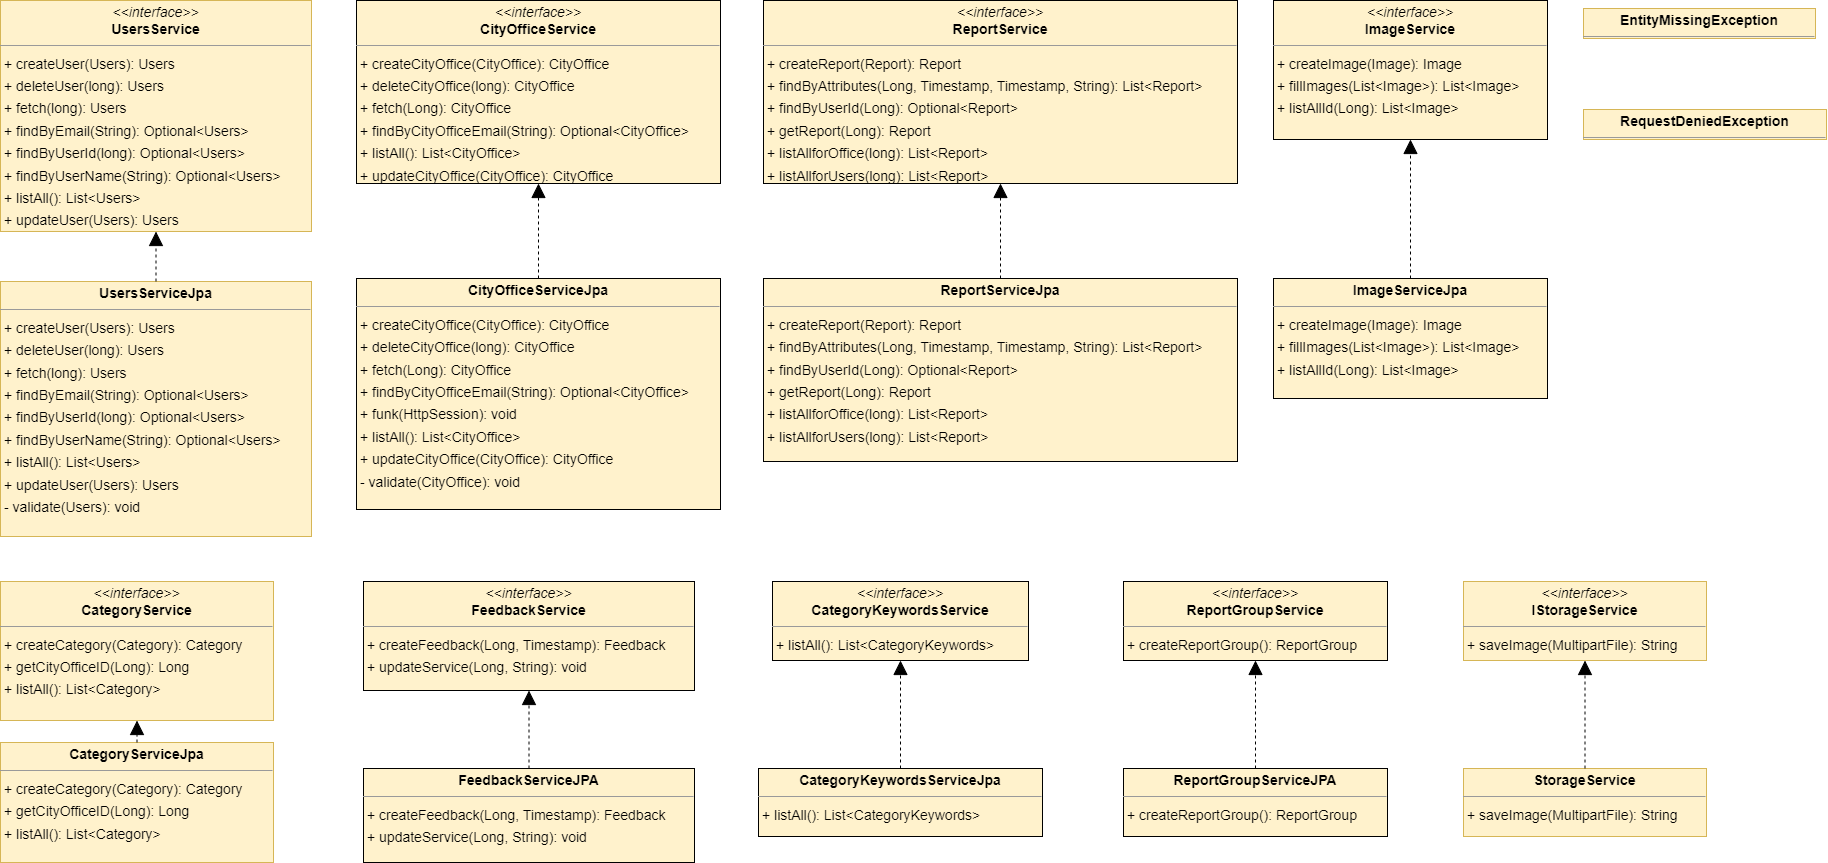
\includegraphics[width=\textwidth]{slike/service.png} %veličina u odnosu na širinu linije
				\caption{Servisi}
				\label{fig:service} %label mora biti drugaciji za svaku sliku
			\end{figure}
		
		
		
		
			\textit{Potrebno je priložiti dijagram razreda s pripadajućim opisom. Zbog preglednosti je moguće dijagram razlomiti na više njih, ali moraju biti grupirani prema sličnim razinama apstrakcije i srodnim funkcionalnostima.}\\
			
			\textbf{\textit{dio 1. revizije}}\\
			
			\textit{Prilikom prve predaje projekta, potrebno je priložiti potpuno razrađen dijagram razreda vezan uz \textbf{generičku funkcionalnost} sustava. Ostale funkcionalnosti trebaju biti idejno razrađene u dijagramu sa sljedećim komponentama: nazivi razreda, nazivi metoda i vrste pristupa metodama (npr. javni, zaštićeni), nazivi atributa razreda, veze i odnosi između razreda.}\\
			
			\textbf{\textit{dio 2. revizije}}\\			
			
			\textit{Prilikom druge predaje projekta dijagram razreda i opisi moraju odgovarati stvarnom stanju implementacije}
			
			
			\eject
			